\chapter{Ondervonden problemen}
\label{Ondervonden_problemen}

\section{Hardware}

\subsection{Voetjes van de printer}

De voetjes van de printer waren te kort, dus daar zijn langere voor
ontworpen en ge 3D print. Zie Figuur ~\ref{fig:voetjes} voor een render van
het 3d ontwerp

\begin{figure}[h]
\centerline{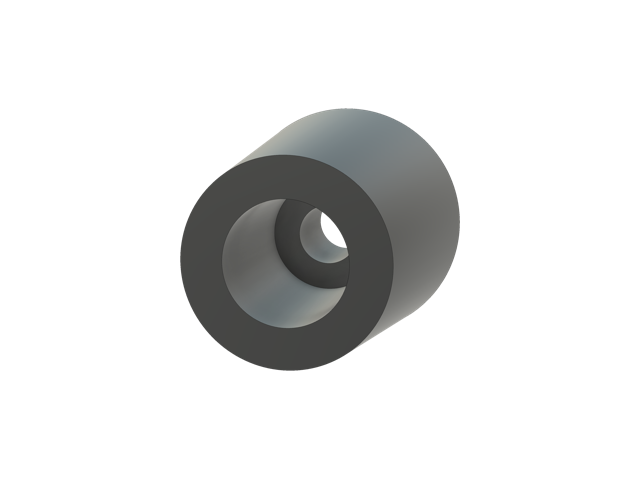
\includegraphics[scale=.5]{voetjes}}
\caption{Render van het 3d ontwerp van de voetjes van de printer}
\label{fig:voetjes}
\end{figure}

\subsection{afstandhouder}

De originele printer is omgebouwd met roestvrijstalen panelen aan alle kanten.
Om ervoor te zorgen dat er goede thermische isolatie is van de print kamer, is
het een dubbelwandig ontwerp met glaswol er tussen. De dubbele wanden worden op
afstand gehouden met ge-3D-printen afstandhouders. Zie Figuur
~\ref{fig:afstandhouder} voor een render van het 3d ontwerp van deze
afstandhouders.

\begin{figure}[h]
\centerline{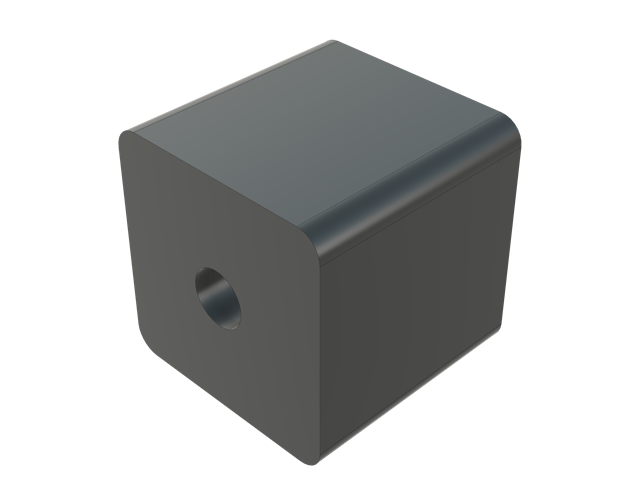
\includegraphics[scale=.5]{afstandhouder}}
\caption{Render van het 3d ontwerp van de afstandhouder van de printer}
\label{fig:afstandhouder}
\end{figure}


\section{Electronica}
\section{Software}
